% Options for packages loaded elsewhere
\PassOptionsToPackage{unicode}{hyperref}
\PassOptionsToPackage{hyphens}{url}
\PassOptionsToPackage{dvipsnames,svgnames,x11names}{xcolor}
%
\documentclass[
  12pt,
  letterpaper,
  DIV=11,
  egregdoesnotlikesansseriftitles]{scrartcl}

\usepackage{amsmath,amssymb}
\usepackage{iftex}
\ifPDFTeX
  \usepackage[T1]{fontenc}
  \usepackage[utf8]{inputenc}
  \usepackage{textcomp} % provide euro and other symbols
\else % if luatex or xetex
  \usepackage{unicode-math}
  \defaultfontfeatures{Scale=MatchLowercase}
  \defaultfontfeatures[\rmfamily]{Ligatures=TeX,Scale=1}
\fi
\usepackage{lmodern}
\ifPDFTeX\else  
    % xetex/luatex font selection
  \setmainfont[]{Palatino Linotype}
\fi
% Use upquote if available, for straight quotes in verbatim environments
\IfFileExists{upquote.sty}{\usepackage{upquote}}{}
\IfFileExists{microtype.sty}{% use microtype if available
  \usepackage[]{microtype}
  \UseMicrotypeSet[protrusion]{basicmath} % disable protrusion for tt fonts
}{}
\makeatletter
\@ifundefined{KOMAClassName}{% if non-KOMA class
  \IfFileExists{parskip.sty}{%
    \usepackage{parskip}
  }{% else
    \setlength{\parindent}{0pt}
    \setlength{\parskip}{6pt plus 2pt minus 1pt}}
}{% if KOMA class
  \KOMAoptions{parskip=half}}
\makeatother
\usepackage{xcolor}
\setlength{\emergencystretch}{3em} % prevent overfull lines
\setcounter{secnumdepth}{-\maxdimen} % remove section numbering
% Make \paragraph and \subparagraph free-standing
\ifx\paragraph\undefined\else
  \let\oldparagraph\paragraph
  \renewcommand{\paragraph}[1]{\oldparagraph{#1}\mbox{}}
\fi
\ifx\subparagraph\undefined\else
  \let\oldsubparagraph\subparagraph
  \renewcommand{\subparagraph}[1]{\oldsubparagraph{#1}\mbox{}}
\fi


\providecommand{\tightlist}{%
  \setlength{\itemsep}{0pt}\setlength{\parskip}{0pt}}\usepackage{longtable,booktabs,array}
\usepackage{calc} % for calculating minipage widths
% Correct order of tables after \paragraph or \subparagraph
\usepackage{etoolbox}
\makeatletter
\patchcmd\longtable{\par}{\if@noskipsec\mbox{}\fi\par}{}{}
\makeatother
% Allow footnotes in longtable head/foot
\IfFileExists{footnotehyper.sty}{\usepackage{footnotehyper}}{\usepackage{footnote}}
\makesavenoteenv{longtable}
\usepackage{graphicx}
\makeatletter
\def\maxwidth{\ifdim\Gin@nat@width>\linewidth\linewidth\else\Gin@nat@width\fi}
\def\maxheight{\ifdim\Gin@nat@height>\textheight\textheight\else\Gin@nat@height\fi}
\makeatother
% Scale images if necessary, so that they will not overflow the page
% margins by default, and it is still possible to overwrite the defaults
% using explicit options in \includegraphics[width, height, ...]{}
\setkeys{Gin}{width=\maxwidth,height=\maxheight,keepaspectratio}
% Set default figure placement to htbp
\makeatletter
\def\fps@figure{htbp}
\makeatother
\newlength{\cslhangindent}
\setlength{\cslhangindent}{1.5em}
\newlength{\csllabelwidth}
\setlength{\csllabelwidth}{3em}
\newlength{\cslentryspacingunit} % times entry-spacing
\setlength{\cslentryspacingunit}{\parskip}
\newenvironment{CSLReferences}[2] % #1 hanging-ident, #2 entry spacing
 {% don't indent paragraphs
  \setlength{\parindent}{0pt}
  % turn on hanging indent if param 1 is 1
  \ifodd #1
  \let\oldpar\par
  \def\par{\hangindent=\cslhangindent\oldpar}
  \fi
  % set entry spacing
  \setlength{\parskip}{#2\cslentryspacingunit}
 }%
 {}
\usepackage{calc}
\newcommand{\CSLBlock}[1]{#1\hfill\break}
\newcommand{\CSLLeftMargin}[1]{\parbox[t]{\csllabelwidth}{#1}}
\newcommand{\CSLRightInline}[1]{\parbox[t]{\linewidth - \csllabelwidth}{#1}\break}
\newcommand{\CSLIndent}[1]{\hspace{\cslhangindent}#1}

\usepackage{fancyhdr}

% Seitenstil festlegen
\pagestyle{fancy}

% Kopfzeile konfigurieren
\lhead{Modul TA.Baustatik I}
\chead{}
\rhead{
\includegraphics[height=0.5cm]{../images/logos/logo-hslu-en-col}}

% Fußzeile konfigurieren
\lfoot{Pascal Gitz}
\cfoot{}
\rfoot{\thepage}


% Überschreibt den Befehl maketitle, da keine Titelseite gewünscht ist
\renewcommand{\maketitle}{}
\KOMAoption{captions}{tableheading}
\makeatletter
\makeatother
\makeatletter
\makeatother
\makeatletter
\@ifpackageloaded{caption}{}{\usepackage{caption}}
\AtBeginDocument{%
\ifdefined\contentsname
  \renewcommand*\contentsname{Inhaltsverzeichnis}
\else
  \newcommand\contentsname{Inhaltsverzeichnis}
\fi
\ifdefined\listfigurename
  \renewcommand*\listfigurename{Abbildungsverzeichnis}
\else
  \newcommand\listfigurename{Abbildungsverzeichnis}
\fi
\ifdefined\listtablename
  \renewcommand*\listtablename{Tabellenverzeichnis}
\else
  \newcommand\listtablename{Tabellenverzeichnis}
\fi
\ifdefined\figurename
  \renewcommand*\figurename{Abbildung}
\else
  \newcommand\figurename{Abbildung}
\fi
\ifdefined\tablename
  \renewcommand*\tablename{Tabelle}
\else
  \newcommand\tablename{Tabelle}
\fi
}
\@ifpackageloaded{float}{}{\usepackage{float}}
\floatstyle{ruled}
\@ifundefined{c@chapter}{\newfloat{codelisting}{h}{lop}}{\newfloat{codelisting}{h}{lop}[chapter]}
\floatname{codelisting}{Listing}
\newcommand*\listoflistings{\listof{codelisting}{Listingverzeichnis}}
\makeatother
\makeatletter
\@ifpackageloaded{caption}{}{\usepackage{caption}}
\@ifpackageloaded{subcaption}{}{\usepackage{subcaption}}
\makeatother
\makeatletter
\@ifpackageloaded{tcolorbox}{}{\usepackage[skins,breakable]{tcolorbox}}
\makeatother
\makeatletter
\@ifundefined{shadecolor}{\definecolor{shadecolor}{rgb}{.97, .97, .97}}
\makeatother
\makeatletter
\makeatother
\makeatletter
\makeatother
\ifLuaTeX
\usepackage[bidi=basic]{babel}
\else
\usepackage[bidi=default]{babel}
\fi
\babelprovide[main,import]{ngerman}
% get rid of language-specific shorthands (see #6817):
\let\LanguageShortHands\languageshorthands
\def\languageshorthands#1{}
\ifLuaTeX
  \usepackage{selnolig}  % disable illegal ligatures
\fi
\IfFileExists{bookmark.sty}{\usepackage{bookmark}}{\usepackage{hyperref}}
\IfFileExists{xurl.sty}{\usepackage{xurl}}{} % add URL line breaks if available
\urlstyle{same} % disable monospaced font for URLs
\hypersetup{
  pdftitle={Testat\_3},
  pdflang={de},
  colorlinks=true,
  linkcolor={blue},
  filecolor={Maroon},
  citecolor={Blue},
  urlcolor={Blue},
  pdfcreator={LaTeX via pandoc}}

\title{Testat\_3}
\author{}
\date{}

\begin{document}
\maketitle
\ifdefined\Shaded\renewenvironment{Shaded}{\begin{tcolorbox}[sharp corners, interior hidden, borderline west={3pt}{0pt}{shadecolor}, enhanced, frame hidden, boxrule=0pt, breakable]}{\end{tcolorbox}}\fi

\hypertarget{testat-3---aufgabenstellung}{%
\section{Testat 3 -
Aufgabenstellung}\label{testat-3---aufgabenstellung}}

\hypertarget{stringer-tafelmodell-und-querschnittswerte}{%
\subsection{Stringer-Tafelmodell und
Querschnittswerte}\label{stringer-tafelmodell-und-querschnittswerte}}

In Anlehnung an das Testat 1 wird ein Stringer-Tafelmodell aus dem
einfachen Balken gebildet. Die Streckenlast ist zu einer Punktlast
vereinfacht worden. Die Einwirkungen sind auf charakteristischem Niveau
\footnote{Charakteristisch bedeutet frei von Sicherheitsbeiwerten. Für
  diese Testatübung ist dies nicht relevant.}.

\begin{figure}[H]

{\centering 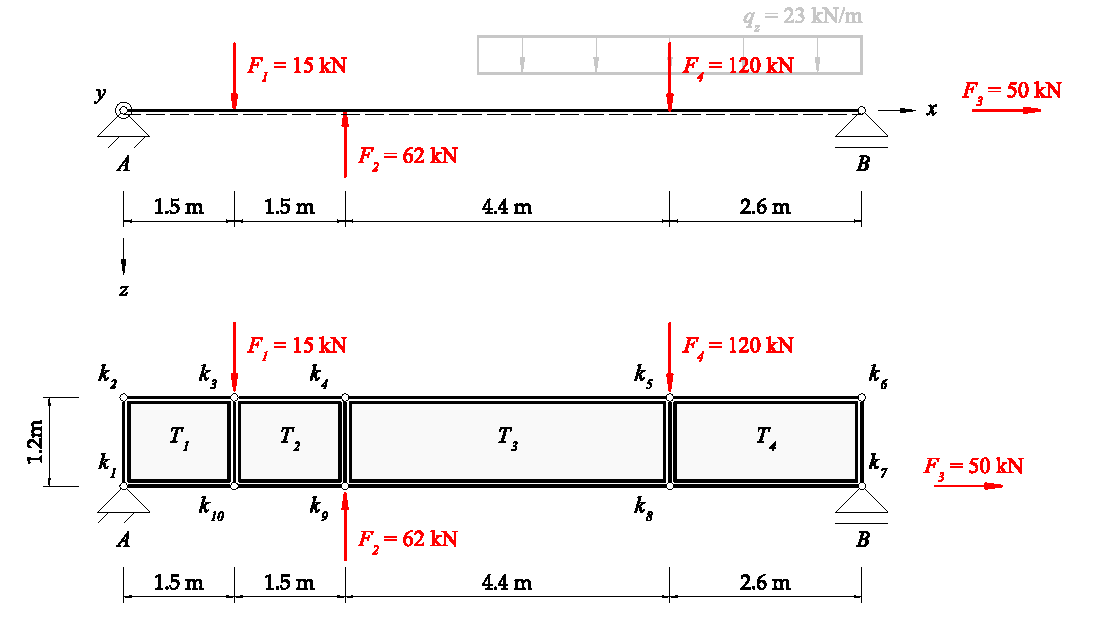
\includegraphics{BSI_HS23_Testat_03_files/mediabag/../images/Testat_03_HS23.pdf}

}

\caption{\label{fig-system}Ein einfacher Balken und Stringer-
Tafelmodell mit Punktlasten}

\end{figure}

Gesucht:

\begin{itemize}
\tightlist
\item
  Beschreiben Sie die statische Bestimmtheit des Stringer-Tafelmodells
\item
  Bestimmen Sie die Lagerkraftgrössen und kontrollieren Sie diese
\item
  Zeichnen Sie die Zustandslinien der Normalkräfte in den Stringern und
  die Schubflüsse in den Tafeln
\end{itemize}

\newpage{}

Unabhängig des Stringertafelmodells gilt es den Querschnitt in
Abbildung~\ref{fig-qs} zu untersuchen:

\begin{figure}[H]

{\centering 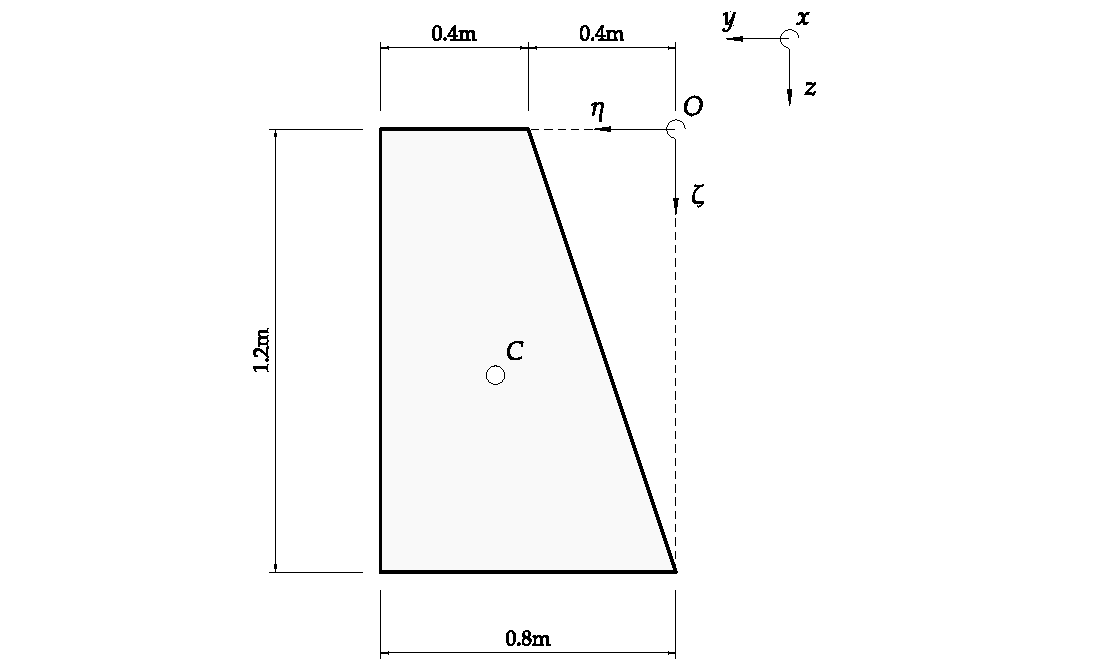
\includegraphics{BSI_HS23_Testat_03_files/mediabag/../images/Testat_03_HS23_QS.pdf}

}

\caption{\label{fig-qs}Ein unsymmetrischer Querschnitt}

\end{figure}

Gesucht:

\begin{itemize}
\tightlist
\item
  Bestimmen Sie den geometrischen Schwerpunkt
\item
  Bestimmen Sie die Hauptwerte der Flächenträgheitsmomente sowie den
  Richtungswinkel
\end{itemize}

\newpage{}

\hypertarget{testat-3---musterluxf6sung}{%
\section{Testat 3 - Musterlösung}\label{testat-3---musterluxf6sung}}

\hypertarget{voraussetzungen}{%
\subsection{Voraussetzungen}\label{voraussetzungen}}

Folgende Annahmen gelten für ein ideales Stringer-Tafelmodell wie in
{[}\protect\hyperlink{ref-Heinzmann2019}{1}{]} definiert:

\begin{itemize}
\tightlist
\item
  die einzelnen Stringer des Stringer-Tafelmodells sind geradlinig
\item
  die Stringer schneiden sich zentrisch in den Knotenpunkten
\item
  die Knoten bilden reibungsfreie Gelenke
\item
  die Belastung ist entweder als Einzelkräfte \(Q\) in den Knoten oder
  verteilten Streckenlasten \(q\) entlang der Stringerlängsrichtung
  möglich
\end{itemize}

\hypertarget{statische-bestimmtheit}{%
\subsection{Statische Bestimmtheit}\label{statische-bestimmtheit}}

Mittels Abzählkriterium nach
{[}\protect\hyperlink{ref-Heinzmann2019}{1}{]} kann die statische
Bestimmtheit ermittelt werden. Wichtig dabei ist, dass das
Abzählkriterium eine notwendige, aber nicht hinreichende Bedingung
darstellt. Zusätzlich ist die kinematische Unverschieblichkeit zu
prüfen.

\begin{equation}n = c - 2 k + s\end{equation}

Dabei sind \(s\) Stringer und Tafeln vorhanden:

\begin{equation}s = 17\end{equation}

und \(k\) Knoten:

\begin{equation}k = 10\end{equation}

sowie \(c\) Lagerkraftgrössen:

\begin{equation}c = 3\end{equation}

Das Abzählkriterium ist eingehalten. Zudem ist das Stringer-Tafelmodell
kinematisch unverschieblich.

\begin{equation}n = 0\end{equation}

\hypertarget{auflagerkruxe4fte}{%
\subsection{Auflagerkräfte}\label{auflagerkruxe4fte}}

\begin{figure}[H]

{\centering 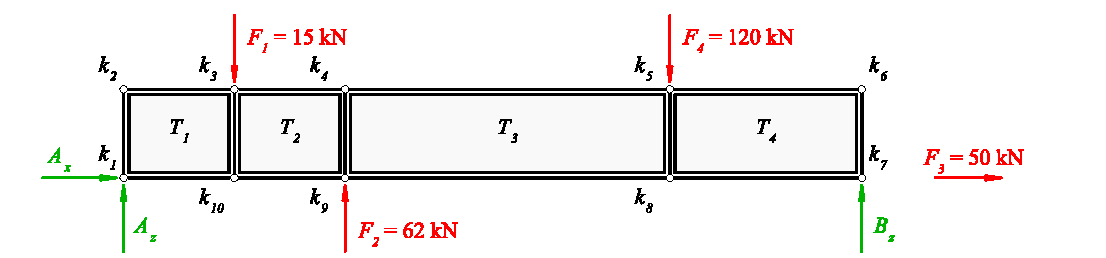
\includegraphics{BSI_HS23_Testat_03_files/mediabag/../images/Testat_03_HS23_SKD.pdf}

}

\caption{\label{fig-system_skd}Stringer-Tafelmodell mit
Lagerkraftgrössen}

\end{figure}

Zuerst wird \(B_z\) ermittelt, dies kann durch Gleichgewicht der Momente
um Punkt \(A\) geschehen.

\begin{equation}\protect\hypertarget{eq-ggw_M_A}{}{
\sum_A^\curvearrowleft M_y = 0
}\label{eq-ggw_M_A}\end{equation}

\begin{equation}0 = B_{z} 10 \text{m} - F_{1} \cdot 1.5 \text{m} + F_{2} \cdot 3 \text{m} - F_{4} \cdot 7.4 \text{m}\end{equation}

\begin{equation}B_{z} = 0.15 F_{1} - 0.3 F_{2} + 0.74 F_{4}\end{equation}

\begin{equation}B_{z} = 72450.0 \text{N}\end{equation}

Anhand des Momentengleichgewichts um Punkt \(B\) kann \(A_z\) ermittelt
werden. \begin{equation}\protect\hypertarget{eq-ggw_M_B}{}{
\sum_B^\curvearrowleft M_y = 0
}\label{eq-ggw_M_B}\end{equation}

\begin{equation}0 = - A_{z} 10 \text{m} + F_{1} \cdot 8.5 \text{m} - F_{2} \cdot 7 \text{m} + F_{4} \cdot 2.6 \text{m}\end{equation}

\begin{equation}A_{z} = 0.85 F_{1} - 0.7 F_{2} + 0.26 F_{4}\end{equation}

\begin{equation}A_{z} = 550.0 \text{N}\end{equation}

Die horizontale Auflagerreaktion \(A_x\) kann durch Gleichgewicht der
horizontalen Kräfte ermittelt werden:

\begin{equation}\protect\hypertarget{eq-sum_fx}{}{
\sum^\rightarrow F_x = 0
}\label{eq-sum_fx}\end{equation}

\begin{equation}0 = A_{x} + F_{3}\end{equation}

\begin{equation}A_{x} = - F_{3}\end{equation}

\begin{equation}A_{x} = - 50000.0 \text{N}\end{equation}

\hypertarget{kontrolle-der-lagerkraftgruxf6ssen}{%
\subsection{Kontrolle der
Lagerkraftgrössen}\label{kontrolle-der-lagerkraftgruxf6ssen}}

Da beide Auflagerkräfte in \(z\)-Richtung mittels eines
Momentengleichgewichts bestimmt worden sind, bleibt die Summe aller
Kräfte in \(z\)-Richtung zur Kontrolle der Grössen.

\begin{equation}\protect\hypertarget{eq-ggw_fz}{}{
\sum^\uparrow F_z = 0
}\label{eq-ggw_fz}\end{equation}

\begin{equation}0 = - A_{z} - B_{z} + F_{1} - F_{2} + F_{4}\end{equation}

\begin{equation}0 = 73000.0 \text{N} - A_{z} - B_{z}\end{equation}

\begin{equation}0 = 0\end{equation}

\hypertarget{zustandslinien-der-schnittgruxf6ssen}{%
\subsection{Zustandslinien der
Schnittgrössen}\label{zustandslinien-der-schnittgruxf6ssen}}

Anhand von Schnittkörperdiagrammen können die Normalkräfte, sowie die
Schubflüsse bestimmt werden.

\hypertarget{bereich-1}{%
\paragraph{Bereich 1}\label{bereich-1}}

Das Schnittkörperdiagramm schneidet unmittelbar links neben dem Knoten.

\begin{figure}[H]

{\centering 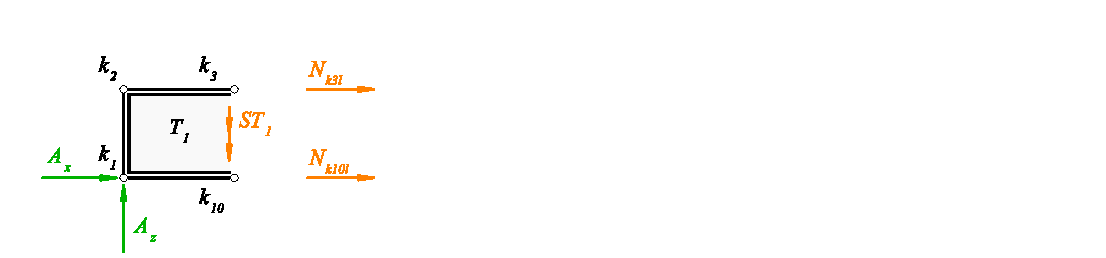
\includegraphics{BSI_HS23_Testat_03_files/mediabag/../images/Testat_03_HS23_SKD4.pdf}

}

\caption{\label{fig-skd1}Schnittkörperdiagramm 1}

\end{figure}

Durch Momentengleichgewicht um \(k_{10}\):

\begin{equation}0 = - A_{z} 1.5 \text{m} - N_{k3l} 1.2 \text{m}\end{equation}

\begin{equation}N_{k3l} = - 1.25 A_{z}\end{equation}

\begin{equation}N_{k3l} = - 687.5 \text{N}\end{equation}

Durch horizontales Gleichgewicht:

\begin{equation}0 = A_{x} + N_{k10l} + N_{k3l}\end{equation}

\begin{equation}N_{k10l} = - A_{x} - N_{k3l}\end{equation}

\begin{equation}N_{k10l} = 50687.5 \text{N}\end{equation}

Durch vertikales Gleichgewicht:

\begin{equation}0 = - A_{z} + ST_{1} \cdot 1.2 \text{m}\end{equation}

\begin{equation}ST_{1} = \frac{0.83 A_{z}}{\text{m}}\end{equation}

\begin{equation}ST_{1} = \frac{458.33 \text{N}}{\text{m}}\end{equation}

\hypertarget{bereich-2}{%
\paragraph{Bereich 2}\label{bereich-2}}

Das Schnittkörperdiagramm schneidet unmittelbar links neben dem Knoten.

\begin{figure}[H]

{\centering 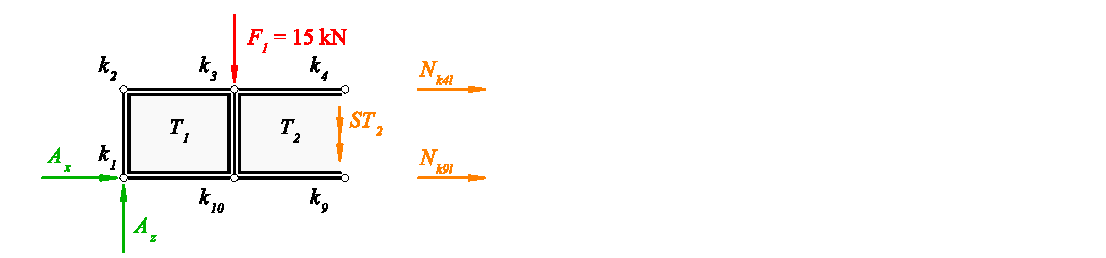
\includegraphics{BSI_HS23_Testat_03_files/mediabag/../images/Testat_03_HS23_SKD3.pdf}

}

\caption{\label{fig-skd2}Schnittkörperdiagramm 2}

\end{figure}

Durch Momentengleichgewicht um \(k_{9}\):

\begin{equation}0 = - A_{z} 3.0 \text{m} + F_{1} \cdot 1.5 \text{m} - N_{k4l} 1.2 \text{m}\end{equation}

\begin{equation}N_{k4l} = - 2.5 A_{z} + 1.25 F_{1}\end{equation}

\begin{equation}N_{k4l} = 17375.0 \text{N}\end{equation}

Durch horizontales Gleichgewicht:

\begin{equation}0 = A_{x} + N_{k4l} + N_{k9l}\end{equation}

\begin{equation}N_{k9l} = - A_{x} - N_{k4l}\end{equation}

\begin{equation}N_{k9l} = 32625.0 \text{N}\end{equation}

Durch vertikales Gleichgewicht:

\begin{equation}0 = - A_{z} + F_{1} + ST_{2} \cdot 1.2 \text{m}\end{equation}

\begin{equation}ST_{2} = \frac{0.83 \left(A_{z} - F_{1}\right)}{\text{m}}\end{equation}

\begin{equation}ST_{2} = - \frac{12042.0 \text{N}}{\text{m}}\end{equation}

\hypertarget{bereich-3}{%
\paragraph{Bereich 3}\label{bereich-3}}

Das Schnittkörperdiagramm schneidet unmittelbar links neben dem Knoten.

\begin{figure}[H]

{\centering 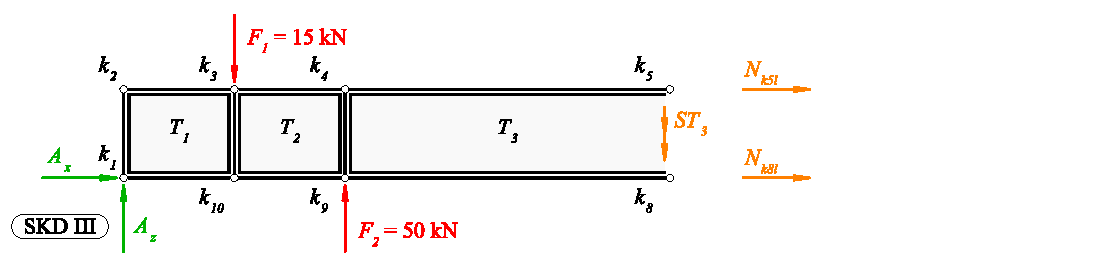
\includegraphics{BSI_HS23_Testat_03_files/mediabag/../images/Testat_03_HS23_SKD2.pdf}

}

\caption{\label{fig-skd3}Schnittkörperdiagramm 3}

\end{figure}

Durch Momentengleichgewicht um \(k_{8}\):

\begin{equation}0 = - A_{z} 7.4 \text{m} + F_{1} \cdot 5.9 \text{m} - F_{2} \cdot 4.4 \text{m} - N_{k5l} 1.2 \text{m}\end{equation}

\begin{equation}N_{k5l} = - 6.17 A_{z} + 4.92 F_{1} - 3.67 F_{2}\end{equation}

\begin{equation}N_{k5l} = - 156975.0 \text{N}\end{equation}

Durch horizontales Gleichgewicht:

\begin{equation}0 = A_{x} + N_{k5l} + N_{k8l}\end{equation}

\begin{equation}N_{k8l} = - A_{x} - N_{k5l}\end{equation}

\begin{equation}N_{k8l} = 206975.0 \text{N}\end{equation}

Durch vertikales Gleichgewicht:

\begin{equation}0 = - A_{z} + F_{1} - F_{2} + ST_{3} \cdot 1.2 \text{m}\end{equation}

\begin{equation}ST_{3} = \frac{0.83 \left(A_{z} - F_{1} + F_{2}\right)}{\text{m}}\end{equation}

\begin{equation}ST_{3} = \frac{39625.0 \text{N}}{\text{m}}\end{equation}

\hypertarget{bereich-4}{%
\paragraph{Bereich 4}\label{bereich-4}}

Das Schnittkörperdiagramm schneidet unmittelbar links neben dem Knoten.

\begin{figure}[H]

{\centering 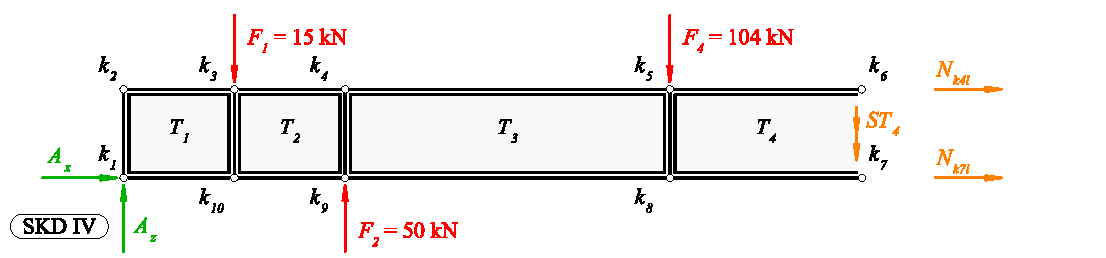
\includegraphics{BSI_HS23_Testat_03_files/mediabag/../images/Testat_03_HS23_SKD1.pdf}

}

\caption{\label{fig-skd4}Schnittkörperdiagramm 4}

\end{figure}

Durch Momentengleichgewicht um \(k_{7}\):

\begin{equation}0 = - A_{z} 10.0 \text{m} + F_{1} \cdot 8.5 \text{m} - F_{2} \cdot 7.0 \text{m} + F_{4} \cdot 2.6 \text{m} - N_{k6l} 1.2 \text{m}\end{equation}

\begin{equation}N_{k6l} = - 8.33 A_{z} + 7.08 F_{1} - 5.83 F_{2} + 2.17 F_{4}\end{equation}

\begin{equation}N_{k6l} = 0\end{equation}

Durch horizontales Gleichgewicht:

\begin{equation}0 = A_{x} + N_{k6l} + N_{k7l}\end{equation}

\begin{equation}N_{k7l} = - A_{x} - N_{k6l}\end{equation}

\begin{equation}N_{k7l} = 50000.0 \text{N}\end{equation}

Durch vertikales Gleichgewicht:

\begin{equation}0 = - A_{z} + F_{1} - F_{2} + F_{4} + ST_{4} \cdot 1.2 \text{m}\end{equation}

\begin{equation}ST_{4} = \frac{0.83 \left(A_{z} - F_{1} + F_{2} - F_{4}\right)}{\text{m}}\end{equation}

\begin{equation}ST_{4} = - \frac{60375.0 \text{N}}{\text{m}}\end{equation}

Der Abschliessende Verlauf lässt sich anhand der Schubflüsse bestimmen.
Beginnend bei einer Puntklast kann anhand des Schubflusses diese entlang
der Tafel angepasst werden. Dies resultiert zu den folgenden
Zustandslinien:

\begin{figure}[H]

{\centering 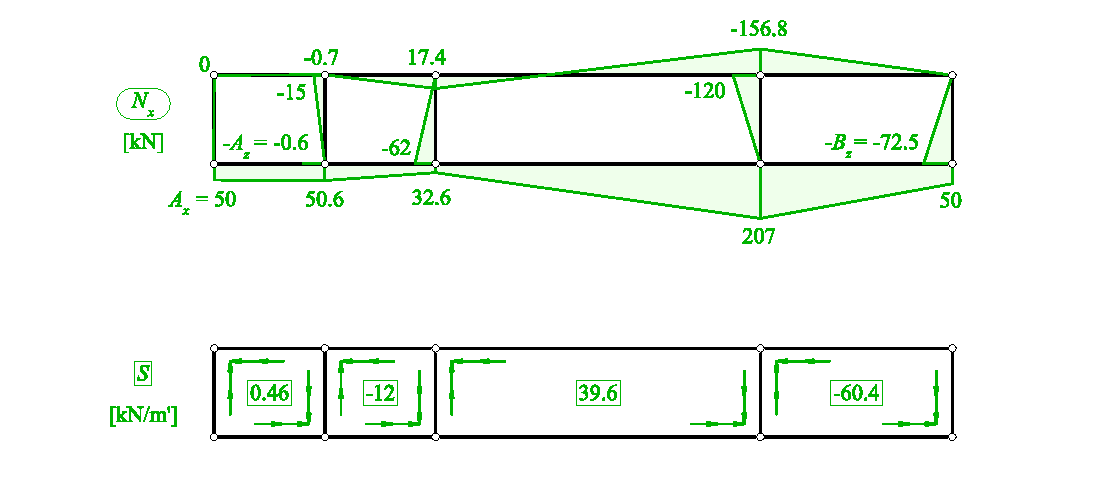
\includegraphics{BSI_HS23_Testat_03_files/mediabag/../images/Testat_03_HS23_N_S.pdf}

}

\caption{\label{fig-ZS_N_S}Zustandslinien der Normalkräfte und der
Schubflüsse}

\end{figure}

\hypertarget{querschnittswerte}{%
\subsection{Querschnittswerte}\label{querschnittswerte}}

Die Bestimmung der Querschnittswerte folgt dem Merkblatt der Vorlesung.
Der Querschnitt in Abbildung~\ref{fig-qs} wird in ein Rechteck und in
ein Dreieck eingeteilt.

\begin{figure}[H]

{\centering 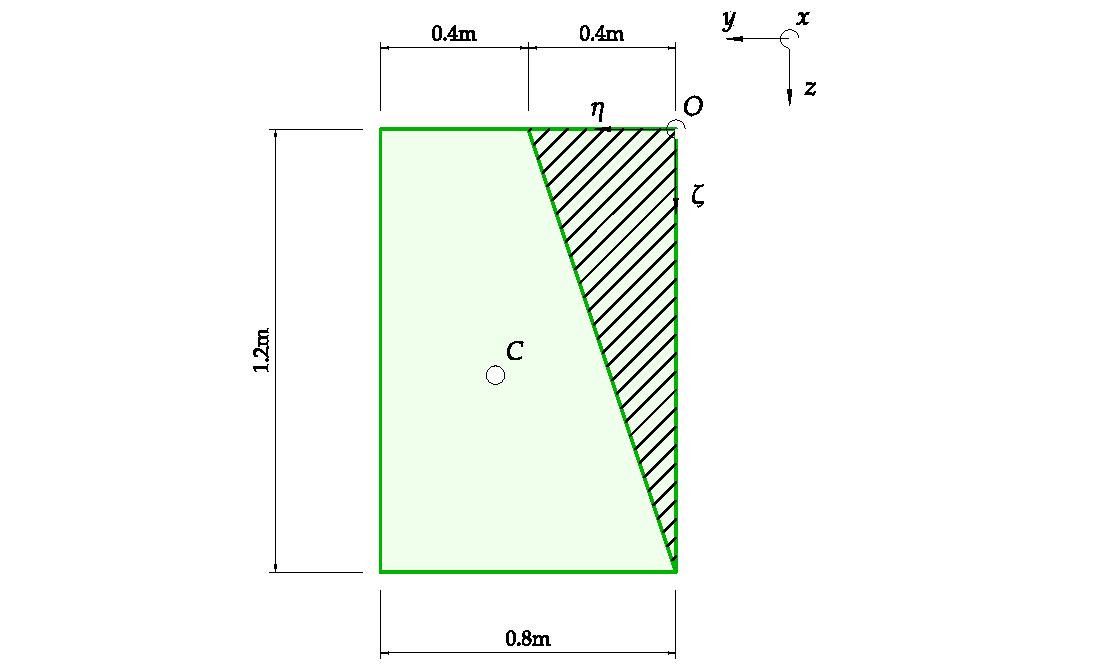
\includegraphics{BSI_HS23_Testat_03_files/mediabag/../images/Testat_03_HS23_QS_aufteilung.pdf}

}

\caption{Aufteilung des Querschnitts in Teilflächen}

\end{figure}

\begin{longtable}[]{@{}
  >{\raggedright\arraybackslash}p{(\columnwidth - 2\tabcolsep) * \real{0.5000}}
  >{\raggedright\arraybackslash}p{(\columnwidth - 2\tabcolsep) * \real{0.5000}}@{}}
\toprule\noalign{}
\endhead
\bottomrule\noalign{}
\endlastfoot
\(b = 0.8 \text{m}\) & \(b_{1} = 0.4 \text{m}\) \\
\(h = 1.2 \text{m}\) & \\
\end{longtable}

\hypertarget{querschnittsfluxe4che}{%
\subsubsection{Querschnittsfläche}\label{querschnittsfluxe4che}}

\begin{equation}A = b h - \frac{b_{1} h}{2}\end{equation}

\begin{equation}A = 0.72 \text{m}^{2}\end{equation}

\hypertarget{fluxe4chenmoment-1.-grades-s_eta-s_zeta}{%
\subsubsection{\texorpdfstring{Flächenmoment 1. Grades \(S_\eta\),
\(S_\zeta\)}{Flächenmoment 1. Grades S\_\textbackslash eta, S\_\textbackslash zeta}}\label{fluxe4chenmoment-1.-grades-s_eta-s_zeta}}

\begin{equation}S_{\eta} = - \frac{h}{3} \frac{b_{1} h}{2} + \frac{h}{2} b h\end{equation}

\begin{equation}S_{\eta} = 0.48 \text{m}^{3}\end{equation}

\begin{equation}S_{\zeta} = \frac{b}{2} b h - \frac{b_{1}}{3} \frac{b_{1} h}{2}\end{equation}

\begin{equation}S_{\zeta} = 0.352 \text{m}^{3}\end{equation}

\hypertarget{lage-des-schwerpunkts-c}{%
\subsubsection{\texorpdfstring{Lage des Schwerpunkts
\(C\)}{Lage des Schwerpunkts C}}\label{lage-des-schwerpunkts-c}}

\begin{equation}\eta_{C} = \frac{S_{\zeta}}{A}\end{equation}

\begin{equation}\eta_{C} = 0.489 \text{m}\end{equation}

\begin{equation}\zeta_{C} = \frac{S_{\eta}}{A}\end{equation}

\begin{equation}\zeta_{C} = 0.667 \text{m}\end{equation}

\hypertarget{fluxe4chenmomente-2.-grades}{%
\subsubsection{Flächenmomente 2.
Grades}\label{fluxe4chenmomente-2.-grades}}

Diese werden anhand des, in den Schwerpunkt verschobenen,
Koordinatensystems ermittelt.

\begin{equation}- 0.133333333333333 \text{m} + \eta_{C} = 0.355558268229167 \text{m}\end{equation}

\begin{equation}- 0.4 \text{m} + \zeta_{C} = 0.2666259765625 \text{m}\end{equation}

\begin{equation}I_{\eta^{'}} = \frac{b h^{3}}{12} + b h \left(- \frac{h}{2} + \zeta_{C}\right)^{2} - \frac{b_{1} h^{3}}{36} - \frac{b_{1} h \left(- \frac{h}{3} + \zeta_{C}\right)^{2}}{2}\end{equation}

\begin{equation}I_{\eta^{'}} = 0.0832 \text{m}^{4}\end{equation}

\begin{equation}I_{\zeta^{'}} = \frac{b^{3} h}{12} + b h \left(- \frac{b}{2} + \eta_{C}\right)^{2} - \frac{b_{1}^{3} h}{36} - \frac{b_{1} h \left(- \frac{b_{1}}{3} + \eta_{C}\right)^{2}}{2}\end{equation}

\begin{equation}I_{\zeta^{'}} = 0.0263 \text{m}^{4}\end{equation}

\begin{equation}C_{\eta^{'}\zeta^{'}} = - b h \left(- \frac{b}{2} + \eta_{C}\right) \left(- \frac{h}{2} + \zeta_{C}\right) - \frac{b_{1}^{2} h^{2}}{72} + \frac{b_{1} h \left(- \frac{b_{1}}{3} + \eta_{C}\right) \left(- \frac{h}{3} + \zeta_{C}\right)}{2}\end{equation}

\begin{equation}C_{\eta^{'}\zeta^{'}} = 0.0139 \text{m}^{4}\end{equation}

\hypertarget{hauptwerte-der-fluxe4chentruxe4gheitsmomente}{%
\subsubsection{Hauptwerte der
Flächenträgheitsmomente}\label{hauptwerte-der-fluxe4chentruxe4gheitsmomente}}

Abschliessend werden die bestimmten Flächenträgheitsmomente in die
Hauptrichtungen transformiert.

\begin{equation}\phi = \frac{\operatorname{atan}{\left(\frac{2 C_{\eta^{'}\zeta^{'}}}{I_{\eta^{'}} - I_{\zeta^{'}}} \right)}}{2}\end{equation}

\begin{equation}\phi = 0.227\end{equation}

\begin{equation}\phi = 13.0 ^\circ\end{equation}

\begin{equation}I_{y} = \frac{I_{\eta^{'}}}{2} + \frac{I_{\zeta^{'}}}{2} + \sqrt{\left(C_{\eta^{'}\zeta^{'}}\right)^{2} + \left(\frac{I_{\eta^{'}}}{2} - \frac{I_{\zeta^{'}}}{2}\right)^{2}}\end{equation}

\begin{equation}I_{y} = 0.0864 \text{m}^{4}\end{equation}

\begin{equation}I_{z} = \frac{I_{\eta^{'}}}{2} + \frac{I_{\zeta^{'}}}{2} - \sqrt{\left(C_{\eta^{'}\zeta^{'}}\right)^{2} + \left(\frac{I_{\eta^{'}}}{2} - \frac{I_{\zeta^{'}}}{2}\right)^{2}}\end{equation}

\begin{equation}I_{z} = 0.0231 \text{m}^{4}\end{equation}

\newpage{}

\hypertarget{literatur}{%
\section*{Literatur}\label{literatur}}
\addcontentsline{toc}{section}{Literatur}

\hypertarget{refs}{}
\begin{CSLReferences}{0}{0}
\leavevmode\vadjust pre{\hypertarget{ref-Heinzmann2019}{}}%
\CSLLeftMargin{1. }%
\CSLRightInline{Heinzmann D (2019) Baustatik 1. Vorlesungsskripte
Hochschule Luzern Technik \& Architektur (HSLU)}

\end{CSLReferences}



\end{document}
